\section{Inverse Functions}\label{sec:InverseFunctions}
In mathematics, an \ifont{inverse} is a function that serves to ``undo'' another function.
That is, if $f(x)$ produces $y$, then putting $y$ into the inverse of $f$ produces the output $x$.
A function $f$ that has an inverse is called invertible and the inverse is denoted by $f^{-1}$.
It is best to illustrate inverses using an arrow diagram:
$$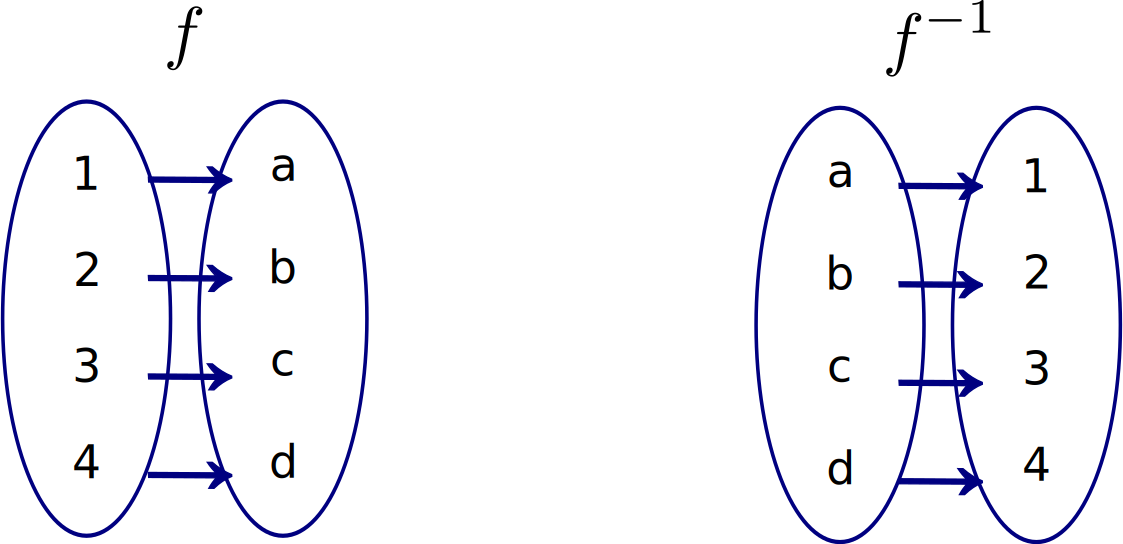
\includegraphics[width=3in]{images/inverse1}$$
Notice how $f$ maps $1$ to $a$, and $f^{-1}$ undoes this, that is, $f^{-1}$ maps $a$ back to $1$.
Don't confuse $f^{-1}(x)$ with exponentiation: the inverse $f^{-1}$ is \ifont{different} from $\frac{1}{f(x)}$.

Not every function has an inverse. It is easy to see that if a 
function $f(x)$ is going to have an inverse, then $f(x)$ 
\ifont{never} takes on the same value twice. We give this property a special name.

A function $f(x)$ is called \dfont{one-to-one}  if every element of the range corresponds to \ifont{exactly} one element of the domain.
Similar to the Vertical Line Test (VLT) for functions, we have the Horizontal Line Test (HLT) for the one-to-one property.

\begin{theorem}{The Horizontal Line Test}{HorizontalLineTest}
A function is one-to-one if and only if there is no horizontal line that intersects its graph more than once.
\end{theorem}

\begin{example}{Parabola is Not One-to-one}{ParabolaNotOneOne}
The parabola $f(x)=x^2$ it not one-to-one because it does not satisfy the horizontal line test.
For example, the horizontal line $y=1$ intersects the parabola at two points, when $x=-1$ and $x=1$.
\end{example}

We now formally define the inverse of a function.

\begin{definition}{Inverse of a Function}{InverseOfAFunction}
Let $f(x)$ and $g(x)$ be two \ifont{one-to-one} functions.
If $(f\circ g)(x)=x$ and $(g\circ f)(x)=x$ then we say 
that $f(x)$ and $g(x)$ are \deffont{inverses} of each other.
We denote $g(x)$ (the inverse of $f(x)$) by $g(x)=f^{-1}(x)$.
\end{definition}

Thus, if $f$ maps $x$ to $y$, then $f^{-1}$ maps $y$ back to $x$.
This gives rise to the \ifont{cancellation formulas}:
$$f^{-1}(f(x))=x,\mbox{\quad for every $x$ in the domain of $f(x)$},$$
$$f(f^{-1}(x))=x,\mbox{\quad for every $x$ in the domain of $f^{-1}(x)$}.$$

\begin{example}{Finding the Inverse at Specific Values}{FindingInverseSpecificValues}
If $f(x)=x^9+2x^7+x+1$, find $f^{-1}(5)$ and $f^{-1}(1)$.
\end{example}

\begin{solution} 
Rather than trying to compute a formula for $f^{-1}$ and then computing $f^{-1}(5)$, we can simply find a number $c$ such that $f$ evaluated at $c$ gives $5$.
Note that subbing in some simple values ($x=-3,-2,1,0,1,2,3$) and evaluating $f(x)$ we eventually find that $f(1)=1^9+2(1^7)+1+1=5$ and $f(0)=1$.
Therefore, $f^{-1}(5)=1$ and $f^{-1}(1)=0$.
\end{solution} 

To compute the equation of the inverse of a function we use the following \ifont{guidelines}.

\begin{formulabox}[Guidelines for Computing Inverses]
\begin{enumerate}\itemsep0pt
	\item Write down $y=f(x)$.
	\item Solve for $x$ in terms of $y$.
	\item Switch the $x$'s and $y$'s.
	\item The result is $y=f^{-1}(x)$.
\end{enumerate}
\end{formulabox}

\begin{example}{Finding the Inverse Function}{FindingInverseFunction}
We find the inverse of the function $f(x)=2x^3+1.$
\end{example}

\begin{solution} 
Starting with $y=2x^3+1$ we solve for $x$ as follows:
$$y-1=2x^3\qquad\to\qquad \frac{y-1}{2}=x^3\qquad\to\qquad x=\sqrt[3]{\frac{y-1}{2}}.$$
Therefore, $\ds f^{-1}(x)=\sqrt[3]{\frac{x-1}{2}}$.
\end{solution}

This example shows how to find the inverse of a function \ifont{algebraically}.
But what about finding the inverse of a function \ifont{graphically}?
Step $3$ (switching $x$ and $y$) gives us a good graphical technique to find the inverse, namely, 
for each point $(a,b)$ where $f(a)=b$, sketch the point $(b,a)$ for the inverse.
More formally, to obtain $f^{-1}(x)$ \ifont{reflect} the graph $f(x)$ about the line $y=x$.

$$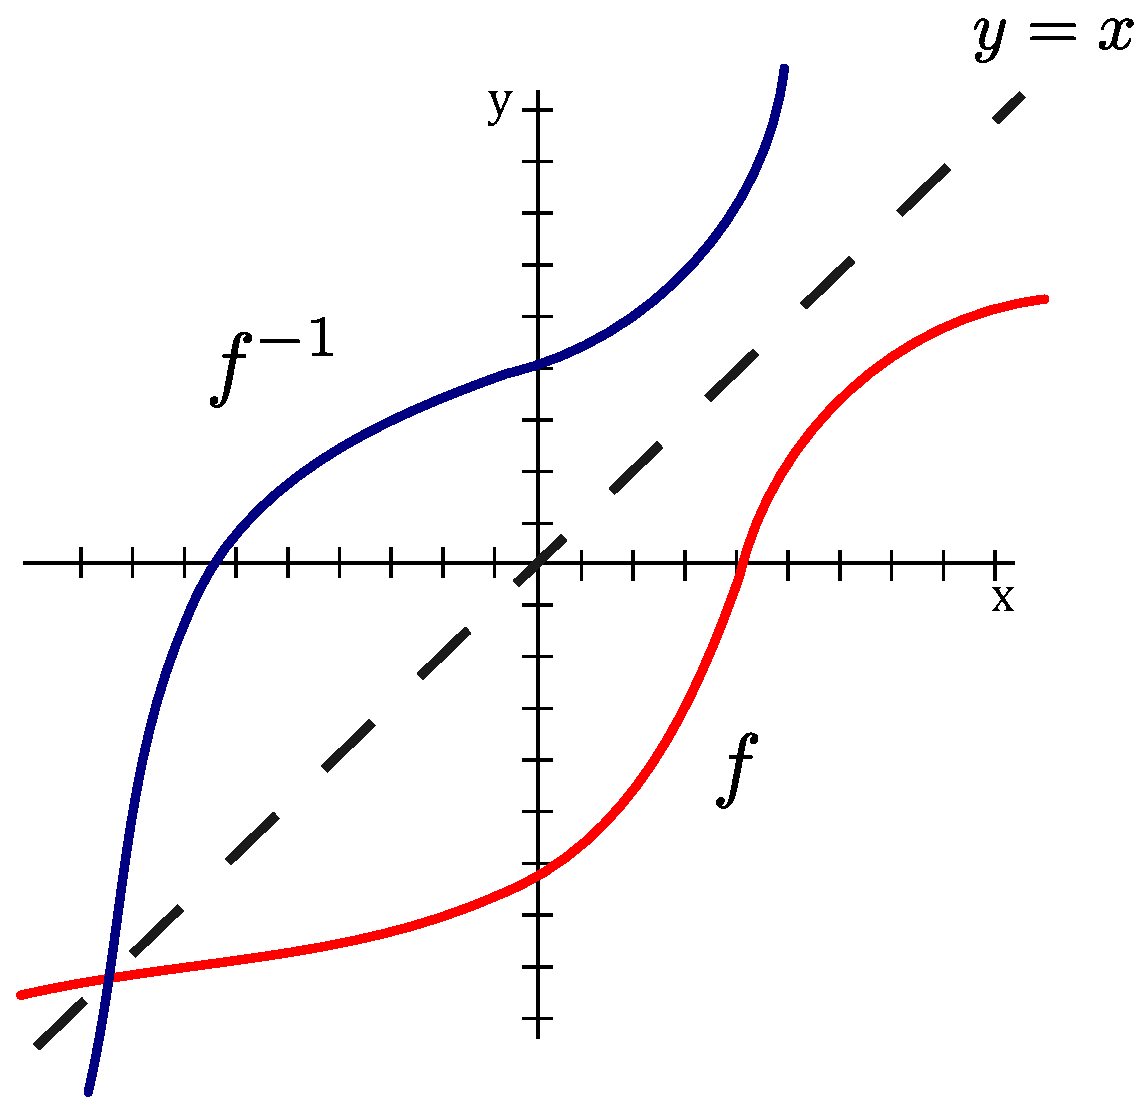
\includegraphics[width=2.5in]{images/inverse2}$$


%%%%%%%%%%%%%%%%%%%%%%%%%%%%%%%%%%%%%%%%%%%%
\Opensolutionfile{solutions}[ex]
\section*{Exercises for \ref{sec:InverseFunctions}}

\begin{enumialphparenastyle}

%%%%%%%%%%
\begin{ex}
Is the function $f(x)=|x|$ one-to-one?
\end{ex}

%%%%%%%%%%
\begin{ex}
If $h(x)=e^x+x+1$, find $h^{-1}(2)$.
\end{ex}

%%%%%%%%%%
\begin{ex}
Find a formula for the inverse of the function $\ds{f(x)=\frac{x+2}{x-2}}$.
\end{ex}

\end{enumialphparenastyle}